\documentclass[parskip=half*]{scrartcl}
\usepackage[spanish, activeacute]{babel}
\usepackage{graphicx, hyperref}
\usepackage{minted}

% CONFIGURACION INICIAL
\title{MulticocoSDL}
\author{Jos\'e Ladislao Lainez Ortega y Jos\'e Molina Colmenero}


%-------------------DOCUMENTO-----------------
\begin{document}
%-------------------PRIMERA PAGINA------------
\maketitle
\vfill
\tableofcontents
\newpage
%---------------------------------------------

%-------------------INTRODUCCION--------------
\section{Introducci\'on}
MulticocoSDL es un juego arcade que emula al famoso Pacman realizado como proyecto para la asignatura Sistemas Multimedia del Grado de Ingenier\'ia Inform\'atica de la Universidad de Ja\'en.

El objetivo de MulticocoSDL es alcanzar varias areas multimedia en un mismo programa haciendo uso de los tres elementos principales del software multimedia:

\begin{description}
	\item[Emplazamiento espacial]	\hfill \\	Los distintos elementos visuales (enemigos, escenario, pacman) son dibujados sobre un canvas en posiciones específicas y además se puede mover por él.
	\item[Control temporal] 		\hfill \\	El jugador puede moverse por el escenario a una determinada velocidad así como los enemigos, estando todos ellos animados.
	\item[Interacci\'on]			\hfill \\	Mediante el teclado el jugador puede dar \'ordenes a pacman de forma que este se mueva en la direcci\'on que el jugador le indica.
\end{description}

El c\'odigo se encuentra alojado en GitHub en el siguiente enlace y contiene un archivo de proyecto de XCode para Mac OS X, si bien el c\'odigo es portable a Windows y Linux. \\

\centerline{\url{https://github.com/L4D15/MulticocoSDL}}

%---------------------------------------------

%-------------------BIBLIOTECAS---------------
\newpage
\section{Bibliotecas}
Se ha hecho uso de la biblioteca Simple DirecMedia Layer as\'i como de algunos subm\'odulos de esta para trabajar con el renderizado de im\'agenes, texto y reproducci\'on de audio. A continuaci\'on explicamos qu\'e tareas ha realizado cada una.

Para m\'as información sobre Simple DirecMedia Layer: \\

\centerline{\url{http://www.libsdl.org/}}

	%---------------SDL-----------------------
	\subsection{SDL}
	Biblioteca con las operaciones b\'asicas para crear una ventana y dibujar en ella. Algunas de las utilidades m\'as usadas han sido:
	\begin{description}
		\item[SDL\_Rect] \hfill \\		Estructura para definir un rect\'angulo. Usado a la hora de recorta un \'area de un SpriteSheet y dibujar en un canvas.
		
		\item[SDL\_Surface] \hfill \\	Superficie o canvas sobre el que dibujar, usado no solo en la ventana principal como contexto de renderizado, sino tambi\'en para almacenar en la memoria de la tarjeta gr\'afica los distintos Sprites a renderizar.
		
		\item[SDL\_BlitSurface(SDL\_Surface*,SDL\_Rect*,SDL\_Surface*,SDL\_Rect*)] \hfill \\ Mediante esta funci\'on se puede dibujar un \'area seleccionada de un canvas origen en un \'area de un canvas de destino. Se ha usado tanto para dibujar en la ventana principal como para separar los distintos Sprites del SpriteSheet.

		\item[SDL\_LoadBMP(const char*)] \hfill \\	Como bien indica su nombre carga una imagen en formato BMP, la guarda en memoria gr\'afica y devuelve un puntero a una SDL\_Surface, de modo que podamos usar la imagen cargada.
	\end{description}

	Esta biblioteca puede descargase desde el siguiente enlace: \\

	\centerline{\url{http://www.libsdl.org/download-1.2.php}}
	%-----------------------------------------
	%---------------SDL_MIXER-----------------
	\subsection{SDL\_Mixer}
	Biblioteca modular de SDL que facilita el trabajo con la reproducci\'on de sonido y m\'usica. Los elementos m\'as destacados de esta biblioteca son:

	\begin{description}
		\item[Mix\_Chunk] \hfill \\	Contenedor de sonido, igual que SDL\_Surface lo era de im\'agenes.

		\item[Mix\_Music] \hfill \\ Contenedor de sonido espec\'ifico para m\'usica.

		\item[Mix\_LoadWAV(const char*)] \hfill \\	Carga un archivo en formato WAV y devuelve un puntero a Mix\_Chunk para poder trabajar con el audio del archivo.

		\item[Mix\_LoadMUS(const char*)] \hfill \\	Carga un archivo en formato WAV, OGG, MP3 o FLAC devolviendo un puntero a Mix\_Music. Esta funci\'on es espec\'ifica para cargar m\'usica ya que SDL\_Mixer trabaja de forma distinta los sonidos y la m\'usica.
	\end{description}

	La biblioteca se puede descargar desde: \\

	\centerline{\url{http://www.libsdl.org/projects/SDL_mixer/}}

	%-----------------------------------------
	%---------------SDL_TTF-------------------
	\subsection{SDL\_TTF}
	A la hora de mostrar la puntuaci\'on del jugador necesit\'abamos mostrar texto por pantalla, por lo que recurrimos a esta biblioteca (otro m\'odulo del proyecto SDL) espec\'ifica para mostrar texto por pantalla. Una curiosidad sobre esta biblioteca es que hace uso de fuentes TTF en lugar de recurrir a fuentes en archivos bitmap como sucede, por ejemplo, al renderizar texto en OpenGL.

	De esta biblioteca hemos usado:

	\begin{description}
		\item[TTF\_Font] \hfill \\	Contenedor para la informaci\'on de la fuente a usar a la hora de renderizar el texto.

		\item[TTF\_OpenFont(const char*, int)] \hfill \\ Carga una fuente desde el archivo en formato TTF especificado y usando el tamaño indicado.

		\item[TTF\_RenderText\_Solid(TTF\_Font, const char*, SDL\_Color)] \hfill \\ Crea una superficie sobre la que dibuja el texto pasado usando la fuente indicada y el color deseado. Una vez tengamos esa superficie habr\'a que dibujarla usando la funci\'on SDL\_BlitSurface(...). 
	\end{description}

	Esta biblioteca est\'a disponible en: \\

	\centerline{\url{http://www.libsdl.org/projects/SDL_ttf/}}
	%-----------------------------------------

%---------------------------------------------

%-------------------IMAGEN--------------------
\newpage
\section{Imagen}
En esta secci\'on explicaremos las clases relacionadas con el apartado visual de la aplicaci\'on, desde la creaci\'on de la ventana hasta la animaci\'on de los personajes que aparecen en pantalla.
	%---------------WINDOW--------------------
	\subsection{Window}
	Antes de poder dibujar nada en pantalla primero necesitamos una ventana para nuestra aplicaci\'on.
		\subsubsection{Inicializaci\'on}
			SDL nos proporciona facilidades a la hora de crear una ventana preparada para renderizar im\'agenes, pero antes de poder usarlas necesitamos inicializar SDL.

			\begin{minted}[frame=lines, samepage=true]{cpp}
int err = SDL_Init(SDL_INIT_AUDIO | SDL_INIT_VIDEO);
    
if (err < 0) {
    // Mostrar error
    std::cout << "Error al inicializar SDL: " << SDL_GetError() << std::endl;
    exit(1);
}
			\end{minted}

			Mediante los flags SDL\_INIT\_AUDIO y SDL\_INIT\_VIDEO le indicamos que nuestra aplicaci\'on va a hacer uso de estas dos funcionalidades. Si no indicaramos, por ejemplo, el flag de audio, nuestra aplicaci\'on no reproducir\'ia audio.

			Si hubiera alg\'un problema durante la incialzaci\'on, SDL puede darnos informaci\'on sobre el fallo mediante SDL\_GetError(). El uso de esta funci\'on para obtener informaci\'on sobre fallos durante el uso de SDL ser\'a una constante a lo largo del proyecto, por lo que se omitir\'a el tratamiento de errores de ahora en adelante. Para m\'as detalles sobre ello consultar el c\'odigo fuente.

			\subsubsection{Creaci\'on}
				Ahora que SDL ya est\'a preparado para funcionar procedemos a crear nuestra ventana.

				\begin{minted}[frame=lines, samepage=true]{cpp}
this->_screen = SDL_SetVideoMode(w, h, 16, SDL_HWSURFACE | SDL_DOUBLEBUF);
				\end{minted}

				Donde \_screen es un SDL\_Surface*, w es la anchura y h la altura de nuestra ventana (y por consiguiente la resoluci\'on en pixeles de nuestro canvas), 16 es la profundidad de bits por pixel (o bpp) y los \'ultimos dos son flags que indican lo siguiente:

				\begin{itemize}
					\item SDL\_HWSURFACE --- La informaci\'on es guardada en la memoria de la gr\'afica, de forma que es m\'as r\'apido trabajar con ella.

					\item SDL\_DOUBLEBUF --- Indica que este canvas tiene doble buffer. Esto es importante para que podamos dibujar sobre un buffer mientras el otro se est\'a mostrando y una vez terminamos de dibujar se intercambian los buffers. De esta forma evitamos que el usuario vea c\'omo se dibujan los elementos poco a poco.
				\end{itemize}

			\subsubsection{Renderizado}
				Una vez la ventana ha sido creada debemos mostrar los elementos que componen el juego. Si bien el m\'etodo render de la clase Windows contiene mucho m\'as c\'odigo, nuestro objetivo aqu\'i es explicar su funcionamiento, por lo que presentamos una versi\'on resumida en la que se renderiza un objeto de ejemplo (clase Entity explicada m\'as adelante) llamado object.

				\begin{minted}[frame=lines, samepage=true]{cpp}
void Window::render()
{
    SDL_FillRect(
    	this->_screen,
    	NULL,
    	SDL_MapRGBA(this->_screen->format, 0, 0, 0, 255)
    );
    object.render(this->_screen);

    SDL_Flip(this->_screen);
}
				\end{minted}

				La primera funci\'on llena el canvas con color negro. Los par\'ametros que se le pasan son una SDL\_Surface*, que ser\'a la superficie a rellenar con color; despu\'es un SDL\_Rect* que indicar\'a el area que queremos rellenar y que al pasarle NULL lo que hace es coger toda el area; y por \'ultimo el color del que queremos rellenar el area, que en este caso ser\'a negro. 

				Despu\'es llamamos al m\'etodo render del objeto al que le pasamos un SDL\_Surface*, es decir, la superficie en la que queremos dibujarlo. Como queremos dibujarlo en la ventana, le pasamos el puntero al canvas creado anteriormente y que tenemos guardado en el atributo \_screen de nuestra clase.

				Por \'ultimo intercambiamos los buffers de la ventana.

			\subsubsection{Eliminaci\'on}
				Hay que tener cuidado al trabajar con las SDL\_Surface pues indicamos a SDL que guarde la informaci\'on visual de nuestra ventana en la memoria gr\'afica. Esto quiere decir que si hicieramos esto:

				\begin{minted}[frame=lines, samepage=true]{cpp}
delete this->_screen;
				\end{minted}

				Estar\'iamos dejando basura en la memoria gr\'afica, ya que delete borra la informaci\'on de la memoria principal, pero no sabe trabajar con la memoria gr\'afica. Es por esto que cuando no necesitemos m\'as una SDL\_Surface se debe liberar usando una funci\'on espec\'ifica de SDL que se encarga tanto de eliminarla de memoria gr\'afica como de memoria principal (la informaci\'on visual, es decir, los pixels, est\'an en memoria gr\'afica, pero otra mucha informaci\'on se guarda en memoria principal tambi\'en).

				Para lidiar con esto hay que declarar los destructores de las clases que hagan uso de alguna SDL\_Surface para que la liberen antes de ser borrados. Mostramos aqu\'i el de la clase Window y omitiremos esta explicaci\'on para el resto de clases.

				\begin{minted}[frame=lines, samepage=true]{cpp}
Window::~Window()
{
    SDL_FreeSurface(this->_screen);
    SDL_Quit();
}
				\end{minted}

				La funci\'on SDL\_Quit() debe llamarse una vez nuestra aplicaci\'on vaya a finalizar y no necesitemos m\'as SDL, pues liberar\'a los recursos que internamente haya reservado cuando lo inicializamos. Como nuestra aplicaci\'on est\'a vinculada a la existencia de la ventana, una vez esta sea destruida debemos ``terminar'' con SDL, por eso se ha incluido en el destructor.

	%-----------------------------------------
	%---------------SPRITE--------------------
	\subsection{Sprite}
		Los Sprites ser\'an las im\'agenes que representen los objetos de nuestro juego. Estos Sprites podr\'an estar animados, para lo cu\'al necesitar\'an una imagen preparada para ello. Nuestra aplicaci\'on soportar\'a Sprites animados siempre y cuando todos los frames tengan las mismas dimensiones.

		\begin{figure}[h]
			\centering
			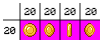
\includegraphics{MulticocoSDL/img/sprite_example.png}
			\caption{Ejemplo de Sprite}
		\end{figure}

		De esta forma a la hora de renderizar el sprite se renderizar\'a solo una secci\'on de la imagen correspondiente al frame actual de la animaci\'on.

		Para manejar esta sistema de animaci\'on necesitamos algo m\'as que simplemente llamar a la funci\'on SDL\_BlitSurface(...) de SDL, y ese es el cometido de la clase Sprite.

		\begin{minted}[frame=lines, samepage=true]{cpp}
class Sprite
{
public:
                    Sprite(SDL_Surface* img, int animations, int w, int h);
                    ~Sprite();
    
    void            render(SDL_Surface* screen, Vector2D& pos);
    void            nextFrame();
    void            setFrameSkip(unsigned int f);
    
private:
    SDL_Surface*    _bitmap;
    unsigned int    _width;
    unsigned int    _height;

    unsigned int    _nAnimations;
    SDL_Rect*       _frames;
    unsigned int    _currentFrame;    
    unsigned int    _frameSkip;
    unsigned int    _framesSkipped;
};
		\end{minted}

		Cada uno de los atributos tiene un cometido espec\'ifico:

		\begin{description}
			\item[\_bitmap] \hfill \\	Contiene la informaci\'on de la imagen guarda en memoria gr\'afica. Se trata de una sola imagen con todos los frames de la animaci\'on.

			\item[\_width y \_height] \hfill \\	Ancho y alto de cada frame individual que componen la animaci\'on.

			\item[\_nAnimations] \hfill \\	N\'umero de frames que componen la animaci\'on.

			\item[\_frames] \hfill \\	Rect\'angulos que corresponden al area de la imagen de cada frame de la animaci\'on. Por ejemplo, si recortamos la imagen \_bitmap usando el rect\'angulo de la primera posici\'on, obtendremos el primer frame de la animaci\'on, si usamos el de la segunda posici\'on, el segundo frame y as\'i sucesivamente.

			\item[\_currentFrame] \hfill \\	Indica en qu\'e frame de la animaci\'on nos encontramos actualmente. De este modo cuando se llame al m\'etodo render se renderizar\'a el frame que corresponde a la animaci\'on actual de forma autom\'atica.

			\item[\_frameSkip y \_frameSkipped] \hfill \\	Usados para controlar la velocidad de animaci\'on. Cuanto mayor sea el frameSkip, m\'as lenta ser\'a la animaci\'on.
		\end{description}

		\subsubsection{Transparencia}
			Veamos c\'omo podemos asignar transparencia al Sprite cuendo se crea:

			\begin{minted}[frame=lines, samepage=true]{cpp}
Sprite::Sprite(SDL_Surface* img, int animations, int w, int h)
{
	// Asignacion de atributos [omitido]
	// ...

	SDL_SetColorKey(
		this->_bitmap,
		SDL_SRCCOLORKEY,
		SDL_MapRGB(this->_bitmap->format,255,0,255)
	);

	// Creacion de los rectangulos de cada frame [omitido]
	//...
}
			\end{minted}

			Nos interesa analizar el uso de SDL\_SetColorKey. Esta funci\'on lo que hace es indicar a la imagen cual es su color clave. El color clave es aquel que se usa como transparencia, de modo que a la hora de dibujar la imagen se dibuja todo menos ese color. En nuestro caso y como se hace en la mayor\'ia de los Sprites de videojuegos hemos usado como color clave un magenta puro, que corresponde con los valores R = 255, G = 0 y B = 255. Se puede ver este color como fondo en la imagen de la moneda presentada anteriormente.

		\subsubsection{Renderizado y animaci\'on}
			Respecto al renderizado y la animaci\'on debemos hablar de dos m\'etodos de la clase Sprite: render y nextFrame.

			\begin{minted}[frame=lines, samepage=true]{cpp}
void Sprite::render(SDL_Surface *screen, Vector2D& pos)
{
    SDL_Rect source = this->_frames[this->_currentFrame];
    SDL_Rect destination;
    destination.x = pos.x();
    destination.y = pos.y();
    destination.w = this->_width;
    destination.h = this->_height;
    
    SDL_BlitSurface(this->_bitmap, &source, screen, &destination);
}
			\end{minted}

			Podemos ver que el rect\'angulo correspondiente con el frame actual (\_currentFrame) se obtiene de la colecci\'on de rect\'angulos que creamos durante el constructor, y el rect\'angulo de destino que define el area donde se dibujar\'a en el canvas de destino se calcula a partir de la posici\'on y del ancho y alto del frame. Despu\'es solo hace falta una llamada a la ya mencionada funci\'on SDL\_BlitSurface(...) y nuestro Sprite se dibujar\'a.

			\textquestiondown Y c\'omo se anima el Sprite si el \'indice \_currentFrame no avanza? Para eso est\'a el m\'etodo nextFrame que hace que la animaci\'on del Sprite avance siguiendo las restricciones impuestas por el frame skip indicado.

			\begin{minted}[frame=lines, samepage=true]{cpp}
void Sprite::nextFrame()
{
    if (this->_framesSkipped == this->_frameSkip) {
        this->_currentFrame = (this->_currentFrame + 1) % this->_nAnimations;
        this->_framesSkipped = 0;
    } else {
        this->_framesSkipped++;
    }
}
			\end{minted}

	%-----------------------------------------
	%---------------SPRITESHEET---------------
	\subsection{SpriteSheet}
		Nuestra clase Sprite solo puede manejar una animaci\'on por Sprite, lo cual nos limita bastante a la hora de animar objetos m\'as complejos que una moneda, como por ejemplo, a Pacman o a los fantasmas. Para ello haremos uso de la clase SpriteSheet que gestionar\'a varios Sprites para un mismo archivo y que adem\'as nos facilitar\'a el manejo de las animaciones.

		\begin{figure}
			\centering
			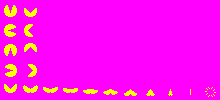
\includegraphics{MulticocoSDL/img/pacman_example.png}
			\caption{Spritesheet de Pacman}
		\end{figure}

		Nuestra clase debe manejar varias animaciones y adem\'as, con n\'umeros de frames distintos.

		\begin{minted}[frame=lines, samepage=true]{cpp}
SpriteSheet::SpriteSheet(const char* img,
			int w, int h,
			int* animations, int nAnimations)
{  
    SDL_Surface* spriteSheet = SDL_LoadBMP(img);    
    SDL_Surface* currentSprite;
    for (int i = 0; i < nAnimations; i++) {
        // Creamos una nueva superficie vacia
        currentSprite = SDL_CreateRGBSurface(
        				SDL_HWSURFACE,
        				w * animations[i], h,
        				16, 0, 0, 0, 0);        
        // Area del SpriteSheet a copiar en el Sprite
        SDL_Rect origin;
        origin.x = 0;
        origin.y = i * h;
        origin.w = w * animations[i];   

        // Dibujamos parte del SpriteSheet
        SDL_BlitSurface(spriteSheet, &origin, currentSprite, NULL);

        // Insertamos un nuevo Sprite en la coleccion
        this->_sprites.push_back(new Sprite(currentSprite,animations[i],w,h));
    }
    SDL_FreeSurface(spriteSheet);    
}
		\end{minted}

		De esta forma hemos dividido la imagen en Sprites que corresponden a cada una de las filas (animaciones) del SpriteSheet.

		\subsubection{Vincular animaciones}
			Tenemos las distintas animaciones del SpriteSheet separadas pero, \textquestiondown C\'omo elegimos qu\'e animaci\'on queremos reproducir? SpriteSheet guarda un \'indice con la posici\'on en la colecci\'on donde se encuentra la posici\'on actual, que ser\'a la que se dibuje si llamamos a SpriteSheet::render(). Dado que este \'indice es un valor num\'erico, debemos conocer la posici\'on dentro de la colecci\'on de la animaci\'on que queremos reproducir. Esto implica que cambiar la animaci\'on actual requerir\'ia saber qu\'e fila corresponde a la animaci\'on en cada SpriteSheet distinto, lo cual puede ser poco intuitivo en cuanto comencemos a trabajar con SpriteSheets distintos.

			Para resolver este problema la clase SpriteSheet
	%-----------------------------------------
%---------------------------------------------

%-------------------AUDIO---------------------
\newpage
\section{Audio}
	%---------------SOUND---------------------
	\subsection{Sound}

	%-----------------------------------------
	%---------------MUSIC---------------------
	\subsection{Music}

	%-----------------------------------------
%---------------------------------------------

%-------------------LÓGICA--------------------
\newpage
\section{L\'ogica}
	%---------------VECTOR2D------------------
	\subsection{Vector2D}

	%-----------------------------------------
	%---------------COLLISIONBOX--------------
	\subsection{CollisionBox}

	%-----------------------------------------

	%-----------------------------------------
	%---------------ENTITY--------------------
	\subsection{Entity}

	%-----------------------------------------
%---------------------------------------------

%-------------------JUEGO---------------------
\newpage
\section{Juego}
	%---------------INICIALIZACIÓN------------
	\subsection{Inicializaci\'on}

	%-----------------------------------------
	%---------------BUCLE PRINCIPAL-----------
	\subsection{Bucle principal}

	%-----------------------------------------
	%---------------EVENTOS-------------------
	\subsection{Eventos}

	%-----------------------------------------
%---------------------------------------------
\end{document}
%---------------------------------------------